\begin{exercise}
      {ID-90260c31646ca54ec6ca9cae367380d06734623f}
      {Kreisverkehr}
  \ifproblem\problem
    Die Fahrbahn eines Kreisverkehrs ist innen \simeter{200} und außen
    \simeter{300} lang. Wie groß ist ihre Fläche?
  \fi
  \ifoutline\outline
    Die Fläche der Fahrbahn erhält man, indem man von der Fläche des
    äußeren Kreises die Fläche des inneren Kreises abzieht:\par
    \begingroup
      \dimen1=4.5cm%
      \begin{minipage}{\dimen1}%
        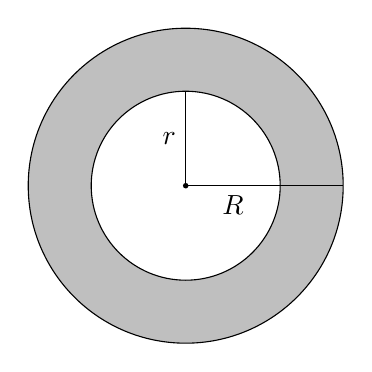
\begin{tikzpicture}%
          \draw[line width=8mm, draw=black!25!white]
               (0, 0) circle[radius=1.6cm];
          \draw (0, 0) circle[radius=1.2cm];
          \draw (0, 0) circle[radius=2.0cm];
          \fill[fill=black] (0, 0) circle[radius=1pt];
          \draw (0, 0) -- node[left]{$r$} +(90:1.2);
          \draw (0, 0) -- node[below, pos=0.3]{$R$} +(0:2.0);
        \end{tikzpicture}%
      \end{minipage}%
      \dimen2=\linewidth%
      \advance\dimen2 by -\dimen1%
      \begin{minipage}{\dimen2}%
        \setlength{\abovedisplayskip}{0pt}%
        \begin{equation*}
          \begin{split}
            U&=2\pi r
            \quad\Rightarrow\quad
            r=\frac{U}{2\pi}
            \\[2ex]
            A&=\pi R^2-\pi r^2
              =\pi\cdot\left(R^2-r^2\right)
          \end{split}
        \end{equation*}
      \end{minipage}%
    \endgroup
  \fi
  \ifoutcome\outcome
    Die Fahrbahn besitzt einen Flächeninhalt von ca. \simm{3978.87}.
  \fi
\end{exercise}
